 \documentclass[c]{beamer}
%\documentclass{beamer}
\listfiles

\mode<presentation>
{
  %\usetheme[deutsch,titlepage0]{KIT}
\usetheme[deutsch]{KIT}
% \usetheme{KIT}

%%  \usefonttheme{structurebold}

  \setbeamercovered{transparent}

  \setbeamertemplate{enumerate items}[circle]
  %\setbeamertemplate{enumerate items}[ball]

}
\usepackage{babel}
\date{}
%\DateText

\newlength{\Ku}
\setlength{\Ku}{1.43375pt}

\usepackage[utf8]{inputenc}
\usepackage[TS1,T1]{fontenc}
\usepackage{array}
\usepackage{multicol}
\usepackage{lipsum}
\usepackage[]{algorithm2e}
\usepackage{amsmath}
\usepackage{color}

\usenavigationsymbols
%\usenavigationsymbols[sfHhdb]
%\usenavigationsymbols[sfhHb]

\subtitle{Algorithmen I SS 14}
\author[]{Lena Winter}

\AuthorTitleSep{\relax}

\institute[ITI]{Institut für Theoretische Informatik}

\TitleImage[width=\titleimagewd]{images/title}

\newlength{\tmplen}

\newcommand{\verysmall}{\fontsize{6pt}{8.6pt}\selectfont}

\title[Algorithmen I SS 14]{Tutorium 4}

\usepackage{alltt}

\TitleImage[height=\titleimageht]{images/sortinghat}

\definecolor{english}{rgb}{0.0, 0.5, 0.0}

\begin{document}

\begin{frame}
  \maketitle
\end{frame}

\begin{frame}{Heaps}
	Eine baumartige Datenstruktur:
	\begin{itemize}
		\item Die Wurzel jedes Subtrees ist in der Ordnungsrelation größer als alle Elemente unter ihm.
		\item Häufige Ordnungen auf Heaps:
		\begin{itemize}
			\item kleiner-gleich: min-Heap
			\item größer-gleich: max-Heap
		\end{itemize}
	\end{itemize}
	\ \\
	\ \\
	\centerline{Im weiteren betrachten wir nur \textbf{Binäre Heaps}}

\end{frame}

\begin{frame} {Heap Operationen}
	\begin{itemize}
		\item Wurzel betrachten in $\mathcal{O}(1)$
		\begin{itemize}
			\item in min-Heaps: das Minimum
			\item in max-Heaps: das Maximum
		\end{itemize}
		\item Heap Eigenschaft herstellen in $\mathcal{O}(n)$
		\item Heap reparieren in $\mathcal{O}(\log  n)$
	\end{itemize}
	Daraus folgt:
	\begin{itemize}
		\item Einfügen in $\mathcal{O}($log $n )$
		\item Wurzel extrahieren in $\mathcal{O}( \log \ n)$
	\end{itemize}

\end{frame}

\begin{frame}{Implementierung}
	Im Computer effizient als Array darstellbar: \\
	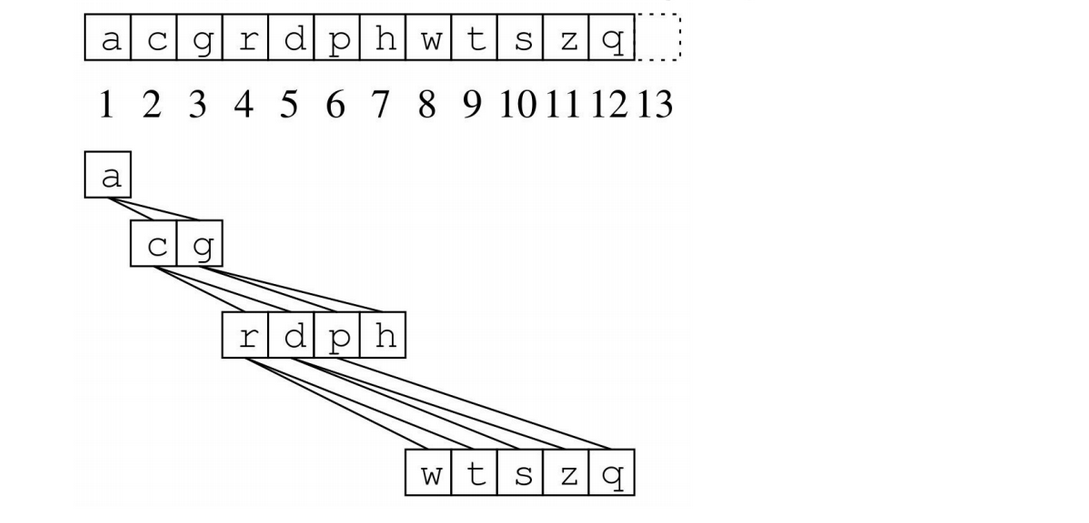
\includegraphics[scale=0.2]{images/heapArray.png} \\
	$\Rightarrow$ Traversierung des Baums?
\end{frame}

\begin{frame}{Baumnavigation in Array Darstellung}
	\begin{description}
		\item[leftChild(i):] heap[$2*i$]
		\item[rightChild(i):] heap[$2*i + 1$]
		\item[parent(i):] heap[$\lfloor i / 2 \rfloor$]
	\end{description}
	\ \\
	\ \\
	Ein Heap der Höhe h hat mindestens $2^{h - 1} $ und maximal $ 2^{h} - 1$ Elemente \\
	\ \\
	Ein Heap mit n Elementen hat die Höhe $\lceil \log_2(n) \rceil$
\end{frame}



\end{document}
